%=====================================================================
%  PROVBIND -- Deliverable Set 2
%  IEEE two-column conference format
%
%  OVERLEAF SETUP
%  1. New Project -> Blank Project
%  2. Upload this file as main.tex
%  3. Upload Project_Dev_Diagram.png into a fig/ folder
%  4. Menu -> Compiler -> pdfLaTeX
%=====================================================================

\documentclass[conference]{IEEEtran}
\IEEEoverridecommandlockouts

\usepackage{cite}
\usepackage{amsmath,amssymb}
\usepackage{graphicx}
\usepackage{xcolor}
\usepackage{tikz}
\usetikzlibrary{arrows.meta,positioning,shapes.geometric}
\usepackage{url}
\usepackage{textcomp}
\usepackage{algorithm}
\usepackage{algpseudocode}
\usepackage{booktabs}

\def\BibTeX{{\rm B\kern-.05em{\sc i\kern-.025em b}\kern-.08em
    T\kern-.1667em\lower.7ex\hbox{E}\kern-.125emX}}

\begin{document}

\title{PROVBIND: Continuous Provenance-Bound Runtime Integrity\\
Verification for Detecting Software Supply Chain Attacks\\
in Cloud-Native Containers}

\author{
\IEEEauthorblockN{Takorn Sripetcharakul, Krittakorn Saetia, Sirasit Wongtawewat,
Panachai Buddharaksa, Somchart Fugkeaw}
\IEEEauthorblockA{Sirindhorn International Institute of Technology,
Thammasat University, Thailand\\
6622771283@g.siit.tu.ac.th, 6622770475@g.siit.tu.ac.th,
6622770426@g.siit.tu.ac.th,\\
6622780664@g.siit.tu.ac.th, somchart@siit.tu.ac.th}
}

\maketitle

%=====================================================================
\begin{abstract}
Software supply chain attacks reach production through legitimate and
fully authorised channels, and container images have become a principal
vehicle for their delivery. Existing defences establish trust before
execution: build frameworks emit signed provenance and a Software Bill
of Materials (SBOM), and admission controllers verify these signatures
before a workload is permitted to start. Such mechanisms prove the
origin of an artifact rather than its trustworthiness, and they establish
trust at a single instant. Runtime monitors observe behaviour
thereafter, but derive their notion of correct behaviour from observed
execution and remain blind to the signed declaration that already
describes what the container was supposed to contain. In this paper we
present PROVBIND, a framework that retains the attestation verified at
admission and compiles it into an expected behavioural envelope
comprising the declared file set with per-layer attribution, the package
dependency closure annotated by depth, and the process closure implied
by the declared entrypoint; a gradient-boosted model supplies capability
and egress expectations where the declaration is silent. An eBPF
collector observes process, file, and network events at kernel level,
and a binding verifier determines for each event whether it contradicts
the declared envelope. Detection is thereby reframed from an
unsupervised statistical problem into a verification problem grounded in
cryptographic evidence: every alert names the specific signed claim it
contradicts, is ranked by the offending component's distance from the
declared dependency closure, and is attributed to the image layer that
introduced it. A separate re-evaluation loop withdraws trust from
already-running workloads when signing key state or external revocation
intelligence changes. Detection results are stored in a graph database
supporting layer attribution and multi-hop deviation correlation.
\end{abstract}

\begin{IEEEkeywords}
software supply chain security, container security, runtime
verification, provenance attestation, eBPF, SBOM
\end{IEEEkeywords}

%=====================================================================
\section{Introduction}

A software supply chain attack reaches its target through a trusted
upstream artifact rather than through a direct intrusion. The adversary
compromises a dependency, a base image, or a build step, which the
target then incorporates and executes on the authority of that trust;
the malicious payload arrives through the same channel as legitimate
software, is signed by the same identities, and is admitted by the same
controls. Contemporary applications are assembled largely from
third-party open-source dependencies and distributed as container images
\cite{mounesan2023}, so a single compromised component can reach
thousands of downstream organisations \cite{ladisa2023,okafor2022}. The
main defence against this is build-time attestation: frameworks such as
SLSA generate signed provenance recording how an artifact was produced,
a Software Bill of Materials (SBOM) enumerates the components it
contains, and tools such as \texttt{cosign} sign the resulting image and
bind these declarations to its content digest
\cite{intoto2019,slsa2023,sigstore2022}.

This defence verifies the wrong property for what happens after
deployment. Admission-time provenance verification establishes
\emph{how an artifact was produced} --- from which source, by which
builder, through which steps --- and confirms that the artifact
presented is the one so produced. It cannot establish whether the
artifact's runtime behaviour stays consistent with that declaration,
since at admission no behaviour has occurred, and the verified
declaration is discarded once the check passes. The 2024 xz-utils
backdoor shows the consequence. A contributor spent roughly two years
building maintainer trust in a compression library present on nearly
every Linux system, then inserted a backdoor; the resulting artifact was
correctly signed, built from the genuine repository by the legitimate
maintainer through the authentic release process, and would satisfy
every attestation-based admission policy deployed today. It was found by
accident, not by any automated control. Vulnerability scanning does not
help, since it detects only catalogued weaknesses and not an
intentionally planted backdoor.

Runtime observation is therefore the remaining line of defence.
Provenance-based intrusion detection systems reconstruct attack
behaviour from system-level event graphs \cite{nodlink2024,orthrus2025},
supply chain specific systems fuse multiple runtime telemetry sources to
reconstruct attack stages \cite{fusechain2026}, and policy-enforcement
systems constrain container behaviour to a profile derived from prior
execution \cite{goleash2025}. Whatever the mechanism, each derives
correct behaviour from observation --- static analysis of code, dynamic
profiling, or statistical learning of a baseline. Behaviour that was
malicious during the learning window is therefore absorbed as normal,
and legitimate but infrequent behaviour is flagged as anomalous
\cite{bilot2025}. None of these systems reads the signed declaration:
the attestation and SBOM that state what the container was built to
contain already exist, but are discarded at admission and never
consulted at runtime.

Using the attestation as a runtime specification takes more than
retaining it. A signed declaration describes an artifact's composition
--- its files, its layers, its package closure --- while runtime
observation yields events, and the two are expressed in different terms.
Compiling one into the other is partly deterministic: the declared file
set comes directly from the image and the package closure directly from
the SBOM, so no declared component can be silently missing. It is partly
not: an SBOM records that a container contains an HTTP client library,
but not that the library needs outbound network access, because
capability and egress requirements appear in no current attestation
format. The declaration is complete about composition and silent about
consequence. A faithful specification must keep the two apart, treating
declaration-derived expectations as authoritative and inferred ones as
advisory rather than mixing signed evidence with prediction.

Trust also has a temporal scope. A container runs for a duration, not an
instant, and may execute for weeks after admission. In that time a
signing key may be disabled, a builder may be found compromised, or an
advisory may be published against a declared component. The transparency
log that anchors the original signature cannot report any of this: it is
append-only and proves only that a signature existed at a given time.

This paper presents PROVBIND, a framework for continuous
provenance-bound runtime integrity verification. Its premise is that
supply chain evidence should not terminate at admission: the signed
declaration establishing what an artifact contains is carried forward
and becomes the specification against which the running artifact is
judged. Our contributions are:

\begin{itemize}
\item \textbf{C1 --- Provenance-to-Runtime Specification Compilation.}
PROVBIND retains signed image provenance and SBOM evidence after
admission and compiles declaration-derived information into an indexed
runtime integrity specification, supplemented by explicitly
distinguished inferred expectations where signed declarations are
silent.

\item \textbf{C2 --- Provenance-Bound Runtime Verification and
Attribution.} Kernel-level runtime events are checked against the
specification, with contradictions linked to the violated declaration
and attributed to the responsible image layer; residual behavioural
analysis separately screens declared-but-atypical behaviour.

\item \textbf{C3 --- Continuous Trust Re-evaluation.} The framework
periodically reassesses the trust state of running workloads against
post-admission changes in key, builder, component, and revocation
status.
\end{itemize}

%=====================================================================
\section{Related Work}

Prior work spans build-time attestation, runtime policy enforcement, and
behavioural detection. We group it by where each approach obtains its
notion of correct behaviour, since that is what separates it from
PROVBIND.

in-toto \cite{intoto2019} provides end-to-end guarantees over the steps
of a build, SLSA \cite{slsa2023} defines build-integrity levels that
culminate in non-falsifiable provenance from a hardened platform, and
Sigstore \cite{sigstore2022} supplies the signing and transparency
infrastructure that made attestation practical at scale, though signing
adoption across public registries remains uneven \cite{schorlemmer2024}.
These establish what an artifact is and where it came from, but verify it
once, before execution.

The gap between SBOM specifications and tool implementations is wide
enough to undermine interoperability \cite{xia2023}, SBOM adoption in
practice remains partial \cite{zahan2023}, and metadata-based SBOM
generation is itself frequently inaccurate \cite{yu2024}. Signed
declarations are increasingly available, then, but are not yet used for
anything beyond admission.

Confine \cite{ghavamnia2020} generates system-call policies by static
analysis of container images, and Optimus \cite{yang2024} filters
system calls dynamically to shrink the attack surface. GoLeash
\cite{goleash2025} profiles package behaviour and enforces per-package
least privilege at package granularity, staying effective under
obfuscation where static analysis fails. Its authors note that code
paths not exercised during profiling are later reported as false
positives at runtime --- the standing limitation of dynamic analysis.

NodLink \cite{nodlink2024} performs online fine-grained detection and
investigation of multi-stage attacks, and ORTHRUS \cite{orthrus2025}
targets the attribution problem that limits provenance-based detection:
detection alone does not localise the responsible entity. A comparison
of state-of-the-art systems finds that simpler configurations often
match elaborate ones \cite{bilot2025}, and a systematization of
container security re-evaluates runtime anomaly detectors on real
vulnerabilities and finds their reported accuracy often overstated
\cite{haq2024}.

Ryu et al. \cite{ryu2026} combine flow-based network metadata with
host-based syscall traces, showing that single-source detection hits
limits hybrid analysis overcomes. FuseChain \cite{fusechain2026} fuses
multiple runtime telemetry sources into temporal provenance graphs to
reconstruct attack stages, with representations learned from benign
traces, and its companion benchmark \cite{synthchain2026} supplies a
multi-source runtime dataset with chain-level ground truth, reporting
that no single telemetry source is chain-complete.

Goyal et al. \cite{goyal2023} show that an adversary able to keep its
behaviour within expected patterns can evade provenance-graph intrusion
detection --- the mimicry case that motivates our residual screening
stage in Section III.

These lines of work are complementary but leave a specific gap, which is
clearest when they are placed side by side. Build-time attestation
\cite{intoto2019,slsa2023,sigstore2022} produces exactly the signed
description of a container's intended composition that a runtime monitor
would need, yet that description is discarded once admission succeeds.
Runtime defences, in turn, reconstruct a notion of correct behaviour
from observation and never consult that description: provenance-based
detectors \cite{nodlink2024,orthrus2025} learn it from event graphs,
supply-chain-specific detectors \cite{fusechain2026} learn it from
benign telemetry, static policy generation \cite{ghavamnia2020} derives
it from code, and dynamic policy enforcement \cite{goleash2025,yang2024}
derives it from profiled executions. Each therefore inherits the
limitation of its evidence source --- learned baselines absorb malicious
behaviour present during training and flag rare-but-legitimate behaviour
\cite{bilot2025}, while profiled policies flag any path not exercised
during profiling \cite{goleash2025} --- and, lacking a signed reference,
none can name which declared claim a given event contradicts.
PROVBIND differs in the origin of its specification: it is neither
learned nor profiled but \emph{read from the signed build declaration
itself}, establishing signed supply chain metadata as a distinct, fourth
source of runtime policy. Because the specification is a declaration
rather than an observation, a violation is a provable contradiction of a
named clause, it is attributable through the declared layer structure to
the base image or build step that introduced it, and it can be
re-evaluated whenever the trust underlying that declaration changes ---
properties that observation-derived detectors cannot provide.

%=====================================================================
\section{Our Proposed System}

\subsection{System Overview}

PROVBIND is organised as a build-time integrity check, verifying admitted
container with a signed attestation, while also performing continuous 
observation and verification stage operating per event, and an independent 
re-evaluation loop to ensure proofs are up to date. 
Fig.~\ref{fig:system} presents our proposed system model.
Each pipeline stage is specified below by an algorithm and the tools
that implement it; Table~\ref{tab:tools} maps stages to tools.

\begin{table}[!t]
\caption{Pipeline stage to implementing tools}
\label{tab:tools}
\centering
\footnotesize
\begin{tabular}{p{0.44\columnwidth}p{0.44\columnwidth}}
\toprule
Stage (algorithm) & Tools \\
\midrule
Build \& signing & BuildKit, syft, cosign, KMS (Vault / cloud), Rekor \\
Attestation retrieval + digest check (Alg.~\ref{alg:retrieve}) &
  Kubernetes watch API, cosign verify, crane \\
Envelope compilation (Alg.~\ref{alg:compile}) &
  Python, \texttt{tarfile}, \texttt{zstandard}, pyelftools/LIEF \\
Capability layer & LightGBM (multi-label) \\
Index construction & Python dict/set, Cuckoo filter \\
Envelope store & Neo4j (K\`uzu embedded fallback) \\
eBPF collection (Alg.~\ref{alg:collect}) & Tetragon \\
Binding verification (Alg.~\ref{alg:verify}) & Python (in-process) \\
Residual screening (Alg.~\ref{alg:residual}) &
  scikit-learn \texttt{IsolationForest} \\
Scoring \& attribution (Alg.~\ref{alg:score}) & Python, Cypher \\
Alert + violation log & \texttt{hashlib} (Merkle), KMS-signed roots, Rekor \\
Trust re-evaluation (Alg.~\ref{alg:retrust}) &
  Rekor client, KMS SDK, OSV/VEX feeds \\
\bottomrule
\end{tabular}
\end{table}

\begin{figure*}[!t]
\centering
\includegraphics[width=\textwidth]{fig/Project_Dev_Diagram.png}
\caption{Our proposed PROVBIND system model. Signed provenance and an
SBOM produced by existing build infrastructure are retained at admission
and compiled into a behavioural envelope; an eBPF collector observes
runtime events, and the binding verifier classifies contradictions of
the envelope, which are scored, attributed to an image layer, and
committed to a hash-chained violation log. A separate timer loop
re-evaluates image trust independently of the event path.}
\label{fig:system}
\end{figure*}

The system model consists of five major parts as follows.

\textit{1) Input data.} A source repository at a specific commit, a
Dockerfile, dependency manifests, and a base image constitute the inputs
to the build. The base image is itself a supply chain input the
developer did not produce, and its layers become layers of the resulting
artifact; this motivates the layer attribution mechanism described in
Section III-C.

\textit{2) Build and signing pipeline.} Continuous integration builds an
image identified by its content digest. An SBOM enumerating the package
closure and an SLSA provenance statement recording source commit, builder
identity, and build parameters are emitted, wrapped in DSSE envelopes,
and signed by the \texttt{cosign} client using a key held in a Key
Management System (KMS) so that private key material never leaves its
hardware boundary. Image and attestations are pushed to a registry, and
a signature record is submitted to the Rekor transparency log. PROVBIND
consumes this stage unchanged.

\textit{3) Admission and compilation.} An admission controller performs
the conventional signature check and admits the pod. Independently and
asynchronously, an attestation retriever fetches the signed documents by
digest and a digest check confirms that the layer digests enumerated in
the manifest match those recorded in the attestation subject. The
envelope compiler then derives the expected behavioural envelope,
assisted by a gradient-boosted model for the capability layer, and
persists it to the database.

\textit{4) Observe and verify.} An eBPF collector on each worker node
captures process execution, file access, and network connection events,
filtering by control group within the kernel. The binding verifier
compares each event against the resident envelope, fronted by a Cuckoo
filter in the node cache. Conforming events are passed to an Isolation
Forest residual screen; contradictions proceed to scoring and
attribution, producing a clause-citing alert recorded in a Merkle-anchored
violation log \cite{merkle1987} whose roots are periodically published
to a transparency log \cite{rfc6962}.

\textit{5) Re-evaluation.} A trust re-evaluator periodically queries KMS
key state, the Rekor inclusion proof, and external revocation feeds,
raising a deviation on the same alert path when trust in an
already-running image no longer holds.

\subsection{Envelope Compilation}

The envelope compiler transforms signed declarations into a
specification against which runtime behaviour can be checked. It
proceeds in four main layers before index construction. The first three
are \emph{declaration-derived}: they are enumerated from the signed
image and SBOM and are complete with respect to what was declared. The
fourth is \emph{inferred}, because no attestation format expresses the
information it supplies. Every entry in the compiled specification
carries this provenance flag, so that an alert can state whether the
expectation it contradicts was signed or predicted, and so that the two
can be evaluated separately.

\textit{1) File layer.} Each image layer is expanded in manifest order.
Whiteout markers are honoured so that files deleted during the build do
not widen the envelope, and for every path both the content hash and the
introducing layer digest are recorded. This layer is fully deterministic
and derives entirely from signed evidence.

\textit{2) Package layer.} The SBOM dependency graph is parsed and each
component assigned a depth by breadth-first traversal from the root
component. Because packages do not execute but files do, each declared
component is additionally resolved to the set of files it installs,
using the package manager records already present in the image; this
file-to-package mapping is what allows an observed event to be
attributed to a component and assigned a dependency depth. A file
covered by no such record is attributable to no declared component and
is treated as maximally distant.

\textit{3) Process layer.} The declared entrypoint is resolved and its
dynamic library closure derived through interpreter directives and
\texttt{DT\_NEEDED} entries. Statically linked binaries expose no such
closure and are covered instead by the file and package layers, a
limitation reported explicitly in our evaluation.

\textit{4) Capability layer (inferred).} No current attestation format
expresses permission or egress requirements. A LightGBM multi-label
classifier
\cite{lightgbm2017}, trained on statically extracted package features
and observed capability usage, predicts the capability set each declared
component requires. The result is intersected with the pod security
context, and the stricter of the two is chosen.

\textit{5) Index construction.} Because per-event verification must be
completed in a fixed time, the supporting structures are derived once
during compilation. A path index maps each declared path to its content
hash and originating layer; a reverse content index maps each hash to
the paths declaring it, distinguishing a binary relocated within the
image from one absent from it entirely; a layer index resolves
attribution by lookup rather than graph traversal; and a depth index
supplies the severity weighting. Compilation and indexing are keyed by
image digest and therefore performed once per distinct image,
irrespective of how many containers are instantiated from it.

\begin{algorithm}[!t]
\footnotesize
\caption{Attestation Retrieval and Digest Check (per pod)}
\label{alg:retrieve}
\begin{algorithmic}[1]
\Require pod event $v$
\Ensure verified bundle, or a deviation
\State $ref \gets v.\text{image}$;\quad $D \gets \textsc{ResolveDigest}(ref)$
  \Comment{never key on a tag}
\State $\textsc{Attach}(v.\text{containerId}, D)$
\If{$D \in \textsc{EnvelopeCache}$}
  \State \Return \Comment{amortised: one compile per digest}
\EndIf
\State $b \gets \textsc{FetchAttestations}(D)$
  \Comment{handles .att/.sig and referrers}
\If{$\neg\,\textsc{VerifySignature}(b, \textsc{PubKey}(b.\text{kmsRef}))$}
  \State \Return $\textsc{Dev}(\textsc{SignatureInvalid}, D)$
\EndIf
\If{$\neg\,\textsc{VerifyInclusion}(b.\text{rekorProof}, \textsc{CurrentSth}())$}
  \State \Return $\textsc{Dev}(\textsc{LogInconsistent}, D)$
\EndIf
\If{$\textsc{LayerDigests}(b.\text{manifest}) \neq \textsc{Subject}(b.\text{attestation})$}
  \State \Return $\textsc{Dev}(\textsc{DigestMismatch}, D)$
\EndIf
\State \Return $b$ \Comment{to Algorithm~\ref{alg:compile}}
\end{algorithmic}
\end{algorithm}

\begin{algorithm}[!t]
\footnotesize
\caption{Envelope Compilation (per image digest)}
\label{alg:compile}
\begin{algorithmic}[1]
\Require digest $D$, attestation $A$, SBOM $B$, manifest $M$, config $C$
\Ensure specification $E$, index set $I$
\If{$\textsc{LayerDigests}(M) \neq \textsc{Subject}(A)$}
  \State \Return $\textsc{Deviation}(\textsc{DigestMismatch})$
\EndIf
\State $F \gets \emptyset$
\ForAll{layer $L \in M.\text{layers}$ \textbf{in manifest order}}
  \ForAll{entry $e \in \textsc{Extract}(L)$}
    \If{$e$ is an opaque marker}
      $F \gets F \setminus \textsc{Subtree}(e.\text{path})$
    \ElsIf{$e$ is a whiteout}
      $F \gets F \setminus \{e.\text{path}\}$
    \Else
      \State $F[e.\text{path}] \gets \langle \textsc{Sha}(e),\,
              L.\text{digest},\, L.\text{index}\rangle$
    \EndIf
  \EndFor
\EndFor
\State $P \gets \textsc{Bfs}(B.\text{deps},\, B.\text{root})$
  \Comment{purl $\mapsto$ depth}
\State $\Phi \gets \textsc{FileToPackage}(F)$
  \Comment{path $\mapsto$ purl}
\State $Q \gets \textsc{Closure}(C.\text{entrypoint})$
  \Comment{declared}
\State $K \gets \textsc{Predict}(P) \cap C.\text{securityContext}$
  \Comment{inferred}
\State $E \gets \langle F,P,\Phi,Q,K\rangle$ with provenance flags
\State $I \gets \langle
  I_{\text{path}}{=}F,\;
  I_{\text{hash}}{=}F^{-1},\;
  I_{\text{layer}},\;
  I_{\text{depth}}{=}P \rangle$
\State \Return $E, I$
\end{algorithmic}
\end{algorithm}

\subsection{Runtime Verification}

\textit{Legitimate runtime state.} A container legitimately creates
state that no build-time declaration can enumerate: temporary files,
caches, logs, sockets, and data written to mounted volumes. The envelope
therefore does not constrain file creation as such. It constrains three
things only: which binaries may be executed, which objects may be loaded
as code into a declared process, and which paths declared by the image
may be modified. Creating a file in a writable path is conforming;
executing it is not. This boundary is what keeps the false positive rate
tractable, since the overwhelming majority of runtime file activity
produces data rather than code.

\textit{Dynamic behaviour.} Three classes require explicit treatment.
Interpreted runtimes load source at execution time through the declared
interpreter rather than through the dynamic loader, so a script
introduced after build appears neither as an execution event nor as a
library load; the envelope covers such a script only where it overwrites
a declared path, and the residual analysis below otherwise applies.
Just-in-time compilation materialises executable pages from data, which
the file layer cannot express, and is instead constrained through the
permissions required to create writable-executable mappings. Runtime
package installation, whether performed by the application or by an
operator, produces files that no signed declaration covers; the
framework reports this as a deviation by construction, on the grounds
that a workload acquiring software after admission has departed from its
attested composition irrespective of intent. Each class is measured
separately, and the resulting false positives are reported by cause
rather than in aggregate.

For each event, container identity resolves to an image digest and
thence to the resident envelope in constant time. Contradictions are
classified into five primary deviation types: undeclared execution,
undeclared library load, write to a path declared immutable by the
image, capability use beyond the declared profile, and undeclared
network egress. Where content hashes are available at execution,
undeclared execution is further refined by the reverse content index
into a modified binary, whose path is declared but whose content is
not, and a relocated binary, whose content is declared but whose path
is not. Conforming events are discarded without further processing,
which is the common case; they are additionally examined by an Isolation
Forest \cite{isoforest2008} that screens the interior of the envelope
for behaviour that is declared but atypical, addressing the adaptive
adversary who confines activity to declared components in order to avoid
contradiction. This residual model is trained on cleared events only and
is distinct in both data and instantiation from the learned anomaly
configuration used as an evaluation baseline.

\begin{algorithm}[!t]
\footnotesize
\caption{eBPF Event Collection (per syscall, in kernel)}
\label{alg:collect}
\begin{algorithmic}[1]
\Require syscall $c$ on hooks
  \{\textsc{Exec}, \textsc{FileOpen}, \textsc{Connect}\}
\Ensure enriched event to userspace, or dropped in kernel
\If{$\textsc{Cgroup}(c) \notin \textsc{MonitoredSet}$}
  \State \textbf{drop} \Comment{in-kernel filter, never crosses}
\EndIf
\If{$c.\text{hook} = \textsc{FileOpen}$ \textbf{and}
     $\neg\,\textsc{WriteIntent}(c.\text{flags})$}
  \State \textbf{drop} \Comment{read-only opens filtered in kernel}
\EndIf
\State $e \gets \textsc{Enrich}(c, \textsc{PodMeta}(c), \textsc{ContainerMeta}(c))$
\State \textbf{emit} $e$ to userspace ring buffer
\end{algorithmic}
\end{algorithm}

\begin{algorithm}[!t]
\footnotesize
\caption{Binding Verification (per event)}
\label{alg:verify}
\begin{algorithmic}[1]
\Require event $v$, index set $I$, specification $E$
\Ensure \textsc{Conforming} or deviation $d$
\State $E,I \gets \textsc{Cache}[\textsc{Digest}(v.\text{container})]$
\If{$v.\text{type} = \textsc{Exec}$}
  \If{$v.\text{path} \in I_{\text{path}}$}
    \If{$v.\text{hash} \neq I_{\text{path}}[v.\text{path}].\text{sha}$}
      \State \Return $\textsc{Dev}(\textsc{ModifiedBinary}, v)$
    \EndIf
    \If{$v.\text{path} \notin Q$}
      \State \Return $\textsc{Dev}(\textsc{UnexpectedProcess}, v)$
    \EndIf
    \State \Return \textsc{Conforming}
  \EndIf
  \If{$v.\text{hash} \in I_{\text{hash}}$}
    \State \Return $\textsc{Dev}(\textsc{RelocatedBinary}, v)$
      \Comment{declared content, undeclared path}
  \EndIf
  \State \Return $\textsc{Dev}(\textsc{UndeclaredExec}, v)$
\ElsIf{$v.\text{type} = \textsc{LibLoad}$ \textbf{and} $v.\text{path} \notin Q$}
  \State \Return $\textsc{Dev}(\textsc{UndeclaredLibrary}, v)$
\ElsIf{$v.\text{type} = \textsc{Write}$ \textbf{and} $v.\text{path} \in I_{\text{path}}$}
  \State \Return $\textsc{Dev}(\textsc{ImmutableWrite}, v)$
    \Comment{creation of new paths is conforming}
\ElsIf{$v.\text{type} = \textsc{Cap}$ \textbf{and} $v.\text{cap} \notin K.\text{caps}$}
  \State \Return $\textsc{Dev}(\textsc{CapabilityExcess}, v)$
\ElsIf{$v.\text{type} = \textsc{Connect}$ \textbf{and} $v.\text{dst} \notin K.\text{egress}$}
  \State \Return $\textsc{Dev}(\textsc{UndeclaredEgress}, v)$
\EndIf
\State \Return \textsc{Conforming}
  \Comment{passed to residual screen}
\end{algorithmic}
\end{algorithm}

\begin{algorithm}[!t]
\footnotesize
\caption{Residual Screening (per conforming event window)}
\label{alg:residual}
\begin{algorithmic}[1]
\Require window $W$ of events returned \textsc{Conforming}
\Ensure low-severity hint, or nothing
\State $x \gets \textsc{Featurise}(W)$
  \Comment{syscall/port/path-class histograms, rates}
\State $s \gets \textsc{IsolationForest}.\textsc{Score}(x)$
  \Comment{node-local, microseconds}
\If{$s < \theta$}
  \State \Return $\textsc{Dev}(\textsc{ResidualAnomaly}, W,\,
                 \text{severity}{=}\textsc{Low})$
\EndIf
\State \Return $\varnothing$
\end{algorithmic}
\end{algorithm}

\subsection{Severity Scoring and Attribution}

Each deviation is weighted by its type and by the depth assigned to the
responsible component during compilation:

\begin{equation}
S \;=\; w_{t}\,\tau(t) \;+\; w_{p}\,\rho(\delta) \;+\; w_{c}\,\kappa,
\qquad w_{t}+w_{p}+w_{c}=1
\end{equation}

\noindent where $\tau(t)\in[0,1]$ weights deviation type $t$,
$\kappa\in[0,1]$ denotes the sensitivity of the capability involved,
and $\rho(\delta)$ is the provenance distance of the component held
responsible for the offending artifact:

\begin{equation}
\rho(\delta) =
\begin{cases}
1 & \text{if } \delta = \bot \quad \text{(no declared component)}\\[4pt]
\dfrac{\delta}{1+\delta} & \text{if } \delta \in \mathbb{N}.
\end{cases}
\end{equation}

Here $\delta$ is the dependency depth recorded during compilation for
the component that installed the offending file, obtained through the
file-to-package mapping of Section III-B; $\delta = 0$ denotes the
application component itself and $\delta = \bot$ an artifact
attributable to no declared component at all. The function is
monotonically increasing in $\delta$ because deep transitive
dependencies receive the least review at build time and are the
predominant vector for upstream compromise, whereas the application's
own code is the least surprising artifact a container can execute.
Since $\rho(\delta) < 1$ for every finite $\delta$, no declared
component can attain the severity of an undeclared artifact at equal
type and capability weight, which is the ranking property the score is
intended to guarantee. Weights are fixed by ablation and reported with
the evaluation.

The violating path is then reverse-resolved through the layer index,
localising the deviation to the image layer that introduced it and
thereby to the base image or build step responsible. Deviations are
grouped by process ancestry within a sliding window so that a
multi-stage compromise is reported as a single chain.
Algorithm~\ref{alg:score} states the procedure.

\begin{algorithm}[!t]
\footnotesize
\caption{Severity Scoring and Attribution (per deviation)}
\label{alg:score}
\begin{algorithmic}[1]
\Require deviation $d$, specification $E$, index set $I$
\Ensure scored, attributed, chained deviation
\State $p \gets \Phi[d.\text{path}]$
  \Comment{responsible component, $\bot$ if none}
\If{$p = \bot$} $\delta \gets \bot$
\Else{} $\delta \gets I_{\text{depth}}[p]$
\EndIf
\State $\rho \gets (\delta = \bot)\;?\;1\;:\;\delta/(1+\delta)$
\State $S \gets w_t\,\tau(d.\text{type}) + w_p\,\rho + w_c\,\kappa(d)$
\State $d.\text{layer} \gets I_{\text{layer}}[d.\text{path}]$
  \Comment{$\bot$ $\Rightarrow$ not from any layer}
\State $d.\text{clause} \gets \textsc{ClauseOf}(d.\text{type}, E, A)$
\State $d.\text{chain} \gets
        \textsc{ChainOf}(d.\text{parentExecId}, \Delta_w)$
\State $d.\text{bucket} \gets \textsc{Bucket}(100 \cdot S)$
\State \Return $d$
\end{algorithmic}
\end{algorithm}

\begin{table}[!t]
\caption{Deviation type weights $\tau(t)$}
\label{tab:tau}
\centering
\footnotesize
\begin{tabular}{lc}
\toprule
Deviation type & $\tau(t)$ \\
\midrule
Undeclared execution      & 1.00 \\
Modified binary           & 1.00 \\
Undeclared library load   & 0.85 \\
Immutable write           & 0.80 \\
Relocated binary          & 0.70 \\
Capability excess         & 0.60 \\
Undeclared egress         & 0.55 \\
Unexpected process        & 0.25 \\
\bottomrule
\end{tabular}
\end{table}

\begin{table}[!t]
\caption{Capability sensitivity $\kappa$ and severity buckets}
\label{tab:kappa}
\centering
\footnotesize
\begin{tabular}{lc@{\qquad}lc}
\toprule
Capability class & $\kappa$ & Bucket & $100\cdot S$ \\
\midrule
Privileged        & 1.00 & Critical & $\geq 80$ \\
Network           & 0.70 & High     & $60$--$79$ \\
Filesystem        & 0.50 & Medium   & $35$--$59$ \\
None              & 0.20 & Low      & $< 35$ \\
\bottomrule
\end{tabular}
\end{table}

Table~\ref{tab:tau} gives the type weights and Table~\ref{tab:kappa} the
capability sensitivities and bucket thresholds. Type weights are ordered
by the strength of the contradiction rather than by perceived
consequence: executing an artifact that appears in no layer of the
attested image, or executing a declared path whose content no longer
matches its declared hash, contradicts the signed declaration outright
and receives the maximum weight. A binary whose content is declared but
whose location is not indicates reuse of an attested executable from an
unexpected path, which is suspicious but not a contradiction of
composition, and is weighted lower. Executing a declared binary outside
the entrypoint closure is the weakest signal, since that closure is an
under-approximation of legitimate behaviour, and is deliberately placed
below the threshold at which an alert would be raised on its own.

Initial weights are $w_t = 0.4$, $w_p = 0.4$, $w_c = 0.2$, fixed by
ablation on benign workloads and reported with the evaluation. Two
illustrative cases show the resulting ordering. An undeclared binary
executed with privileged capability and attributable to no declared
component scores $0.4(1.00) + 0.4(1.00) + 0.2(1.00) = 1.00$, or $100$,
and is bucketed critical. A capability excess by a declared transitive
dependency at depth two, involving only filesystem capability, scores
$0.4(0.60) + 0.4(0.67) + 0.2(0.50) = 0.61$, or $61$, and is bucketed
high. The gap between them is produced principally by $\rho$, which is
the intended behaviour of the metric.

\subsection{Continuous Trust Re-evaluation}

Trust granted at admission is re-examined on a fixed interval
$\Delta t$, independently of the event path.
Algorithm~\ref{alg:retrust} states the procedure. The transparency log
supplies the immutable timestamp anchor against which the signing
history is checked, but not the revocation signal itself, which
originates from the key management service and from external
intelligence. A signature produced before a key was disabled is treated
according to a configured policy: retained where the key was rotated for
operational reasons, invalidated where it was disabled following
compromise. Deviations raised here enter the same alert path as runtime
contradictions and are scored by the same metric, with $\delta$ taken
from the revoked component's recorded depth.

\begin{algorithm}[!t]
\footnotesize
\caption{Continuous Trust Re-evaluation (every $\Delta t$)}
\label{alg:retrust}
\begin{algorithmic}[1]
\ForAll{running image digest $D$}
  \State $A \gets \textsc{Attestation}[D]$
  \If{$\neg\,\textsc{VerifyInclusion}(A.\text{proof},
        \textsc{CurrentSth}())$}
    \State $\textsc{Raise}(\textsc{LogInconsistent}, D)$
  \EndIf
  \State $\sigma \gets \textsc{KeyState}(A.\text{kmsRef})$
  \If{$\sigma \neq \textsc{Enabled}$}
    \State $\textsc{Raise}(\textsc{KeyRevoked}, D)$
  \ElsIf{$A.\text{signTime} > \textsc{DisableTime}(A.\text{kmsRef})$}
    \State $\textsc{Raise}(\textsc{SignedAfterDisable}, D)$
  \EndIf
  \If{$A.\text{builderId} \in \textsc{Denylist}()$}
    \State $\textsc{Raise}(\textsc{BuilderRevoked}, D)$
  \EndIf
  \ForAll{$purl \in E[D].P$}
    \If{$purl \in \textsc{AdvisoryFeed}()$}
      \State $\textsc{Raise}(\textsc{ComponentRevoked},
              D,\, \delta{=}P[purl])$
    \EndIf
  \EndFor
\EndFor
\end{algorithmic}
\end{algorithm}

\subsection{Graph Database Model}

Detection results and the compiled envelopes are stored in a graph
database, whose schema is shown in Fig.~\ref{fig:graph}.

\begin{figure}[!t]
\centering
\resizebox{\columnwidth}{!}{%
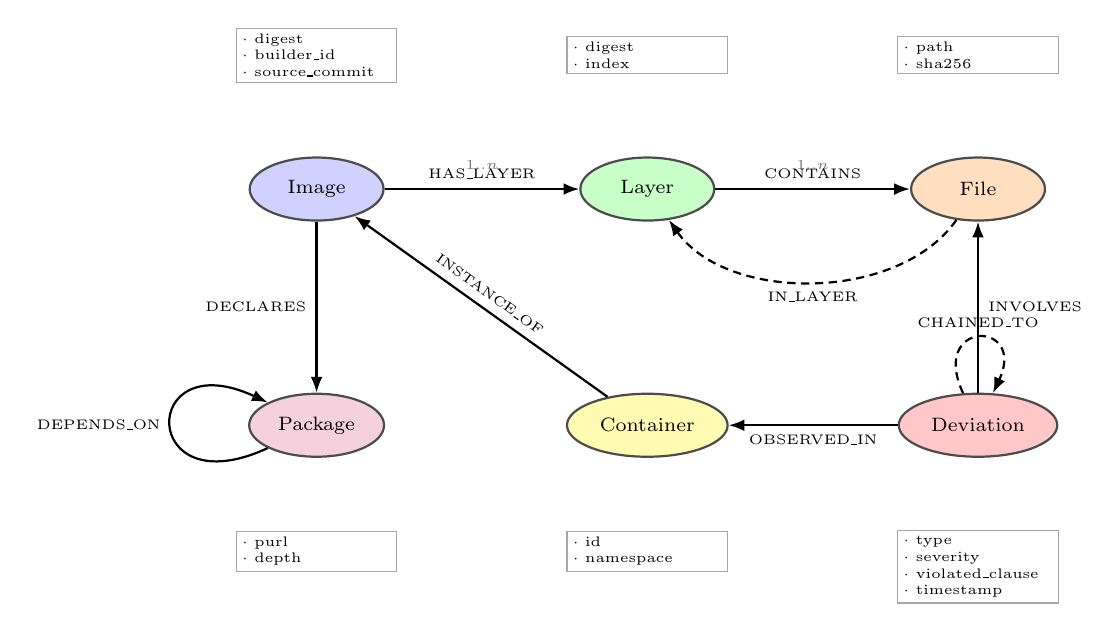
\begin{tikzpicture}[
  font=\scriptsize,
  ent/.style={ellipse, draw=black!70, thick, minimum width=17mm,
              minimum height=8mm, align=center},
  prop/.style={rectangle, draw=black!35, align=left, inner sep=2pt,
               font=\tiny, text width=19mm},
  rel/.style={-{Latex[length=2mm]}, thick, font=\tiny},
  reld/.style={-{Latex[length=2mm]}, thick, font=\tiny, densely dashed}
]

% wider column spacing to stop label overlap
\node[ent, fill=blue!18]   (img) at (0,0)      {Image};
\node[ent, fill=green!22]  (lay) at (4.2,0)    {Layer};
\node[ent, fill=orange!25] (fil) at (8.4,0)    {File};

\node[ent, fill=purple!18] (pkg) at (0,-3.0)   {Package};
\node[ent, fill=yellow!30] (con) at (4.2,-3.0) {Container};
\node[ent, fill=red!22]    (dev) at (8.4,-3.0) {Deviation};

\draw[rel] (img) -- node[above]{HAS\_LAYER} (lay);
\draw[rel] (lay) -- node[above]{CONTAINS}   (fil);
\draw[rel] (img) -- node[left]{DECLARES}    (pkg);
\draw[rel] (con) -- node[above,sloped]{INSTANCE\_OF} (img);
\draw[rel] (pkg) to[out=205,in=155,looseness=8]
      node[left]{DEPENDS\_ON} (pkg);

\draw[rel] (dev) -- node[right]{INVOLVES}     (fil);
\draw[rel] (dev) -- node[below]{OBSERVED\_IN} (con);

% attribution edge, routed low and clear of INVOLVES
\draw[reld] (fil) to[out=235,in=305,looseness=0.9]
      node[below]{IN\_LAYER} (lay);

% chain self-edge, top of Deviation, clear of the right margin
\draw[reld] (dev) to[out=115,in=65,looseness=7]
      node[above]{CHAINED\_TO} (dev);

\node[font=\tiny,black!55] at (2.1,0.30) {1..$n$};
\node[font=\tiny,black!55] at (6.3,0.30) {1..$n$};

\node[prop] at (0,1.7)    {$\cdot$ digest\\$\cdot$ builder\_id\\$\cdot$ source\_commit};
\node[prop] at (4.2,1.7)  {$\cdot$ digest\\$\cdot$ index};
\node[prop] at (8.4,1.7)  {$\cdot$ path\\$\cdot$ sha256};
\node[prop] at (0,-4.6)   {$\cdot$ purl\\$\cdot$ depth};
\node[prop] at (4.2,-4.6) {$\cdot$ id\\$\cdot$ namespace};
\node[prop] at (8.4,-4.8) {$\cdot$ type\\$\cdot$ severity\\$\cdot$ violated\_clause\\$\cdot$ timestamp};

\end{tikzpicture}}
\caption{Graph data model for provenance-bound verification.}
\label{fig:graph}
\end{figure}

The model features six interconnected entities. \textit{(1) Image}
represents an attested container image identified by its content digest,
and carries the builder identity and source commit recorded in the
provenance. \textit{(2) Layer} represents an individual filesystem layer
and its ordinal position within the image, linked through the
\texttt{HAS\_LAYER} relationship. \textit{(3) File} represents a
declared path together with its content hash. Because base layers are
shared across images, \texttt{Layer} and \texttt{File} nodes are keyed
by layer digest and referenced by every image that includes them, so the
graph grows with the number of distinct layers rather than with the
number of images. A \texttt{File} is linked to its introducing layer
both structurally, through \texttt{CONTAINS}, and for attribution,
through \texttt{IN\_LAYER}, which the scoring stage traverses from a
\texttt{Deviation} to localise a violation to the base image or build
step responsible. \textit{(4) Package} represents a declared component
identified by package URL and annotated with its depth from the root
component, with \texttt{DEPENDS\_ON} edges reproducing the SBOM
dependency graph. \textit{(5) Container} represents a running instance
of an image. \textit{(6) Deviation} represents a detected contradiction,
characterised by its type, severity, the attestation clause it violates,
and the moment of detection.

The graph is queried only after a violation has been raised; no database
access occurs on the per-event path. This separation is essential to the
overhead characteristics of the system, since a graph query inside the
event handler would dominate the cost of verification itself.

%=====================================================================
\section{Evaluation Plan}

Detection quality is assessed against ground-truth labels with a supply
chain violation as the positive class, reporting precision, recall,
$F_1$, false positive rate, and accuracy. False positive rate is
reported alongside the $F$-measure rather than folded into it, because
the central claim concerns precision specifically: verification against
a signed specification should eliminate the class of false alarms
arising when a learned baseline encounters legitimate but infrequent
behaviour.

Published corpora supply runtime telemetry and chain-level ground truth
but were assembled to evaluate detectors consuming telemetry alone, and
ship without the signed provenance and SBOM documents this framework
requires; the majority of their scenarios are additionally not
containerised \cite{synthchain2026}. The attack semantics are therefore
extracted and re-instantiated within an attested container testbed, and
this reconstruction is reported explicitly as part of the methodology.

The framework is compared against a rule-based runtime monitor, an
independently trained learned-anomaly detector, and admission-time
signature verification alone. Cost is measured on equal footing with
accuracy: per-event verification latency, node-level CPU and memory
overhead, kernel ring buffer drop rate under burst load, and compilation
and indexing time per image. Overhead is reported relative to existing
runtime collection rather than to an unmonitored host, since the kernel
collection cost is inherited rather than introduced.

%=====================================================================
\begin{thebibliography}{00}

\bibitem{mounesan2023} M. Mounesan, H. Siadati, and S. Jafarikhah,
``Exploring the threat of software supply chain attacks on
containerized applications,'' in \textit{Proc. 16th Int. Conf. Security
of Information and Networks (SIN)}, 2023, pp. 1--8.

% --- SBOM (peer-reviewed) ---

\bibitem{ladisa2023} P. Ladisa, H. Plate, M. Martinez, and O. Barais,
``SoK: Taxonomy of attacks on open-source software supply chains,'' in
\textit{Proc. IEEE Symp. Security and Privacy (S\&P)}, 2023,
pp. 1509--1526.

\bibitem{okafor2022} C. Okafor, T. R. Schorlemmer, S. Torres-Arias, and
J. C. Davis, ``SoK: Analysis of software supply chain security by
establishing secure design properties,'' in \textit{Proc. ACM Workshop
on Software Supply Chain Offensive Research and Ecosystem Defenses
(SCORED)}, 2022, pp. 15--24.

\bibitem{intoto2019} S. Torres-Arias, H. Afzali, T. K. Kuppusamy,
R. Curtmola, and J. Cappos, ``in-toto: Providing farm-to-table
guarantees for bits and bytes,'' in \textit{Proc. 28th USENIX Security
Symp.}, 2019.

\bibitem{slsa2023} Open Source Security Foundation, ``Supply-chain
levels for software artifacts (SLSA), version 1.0 specification,''
OpenSSF, 2023.

\bibitem{sigstore2022} Z. Newman, J. S. Meyers, and S. Torres-Arias,
``Sigstore: Software signing for everybody,'' in \textit{Proc. ACM
SIGSAC Conf. Computer and Communications Security (CCS)}, 2022,
pp. 2353--2367.

\bibitem{nodlink2024} S. Li, F. Dong, X. Xiao, H. Wang, F. Shao,
J. Chen, Y. Guo, X. Chen, and D. Li, ``NodLink: An online system for
fine-grained APT attack detection and investigation,'' in \textit{Proc.
Network and Distributed System Security Symp. (NDSS)}, 2024.

\bibitem{orthrus2025} B. Jiang et al., ``ORTHRUS: Achieving high
quality of attribution in provenance-based intrusion detection
systems,'' in \textit{Proc. 34th USENIX Security Symp.}, 2025.

\bibitem{fusechain2026} University of Glasgow, ``FuseChain: Runtime
evidence reconstruction for software supply-chain attacks,''
\textit{arXiv preprint} arXiv:2606.15811, 2026.

\bibitem{goleash2025} L. Bello, M. Ferrari, and colleagues,
``GoLeash: Mitigating Golang software supply chain attacks with runtime
policy enforcement,'' \textit{arXiv preprint} arXiv:2505.11016, 2025.

\bibitem{bilot2025} T. Bilot, B. Jiang, Z. Li, N. El Madhoun,
K. Al Agha, A. Zouaoui, and T. Pasquier, ``Sometimes simpler is better:
A comprehensive analysis of state-of-the-art provenance-based intrusion
detection systems,'' in \textit{Proc. 34th USENIX Security Symp.},
2025.

\bibitem{schorlemmer2024} T. R. Schorlemmer, K. G. Kalu, L. Chigges,
K. M. Ko, E. A. Ishgair, S. Bagchi, S. Torres-Arias, and J. C. Davis,
``Signing in four public software package registries: Quantity,
quality, and influencing factors,'' in \textit{Proc. IEEE Symp.
Security and Privacy (S\&P)}, 2024, pp. 1160--1178.

\bibitem{xia2023} B. Xia, T. Bi, Z. Xing, Q. Lu, and L. Zhu, ``An
empirical study on software bill of materials: Where we stand and the
road ahead,'' in \textit{Proc. IEEE/ACM 45th Int. Conf. Software
Engineering (ICSE)}, 2023, pp. 2630--2642.

\bibitem{zahan2023} N. Zahan, E. Lin, M. Tamanna, W. Enck, and
L. Williams, ``Software bills of materials are required. Are we there
yet?,'' \textit{IEEE Security \& Privacy}, vol. 21, no. 2,
pp. 82--88, 2023.

\bibitem{yu2024} S. Yu, W. Song, X. Hu, and H. Yin, ``On the
correctness of metadata-based SBOM generation: A differential analysis
approach,'' in \textit{Proc. 54th Annu. IEEE/IFIP Int. Conf. Dependable
Systems and Networks (DSN)}, 2024, pp. 29--36.

% --- container security systematization and runtime defence (peer-reviewed) ---

\bibitem{ghavamnia2020} S. Ghavamnia, T. Palit, A. Mishra, and
M. Polychronakis, ``Confine: Automated system call policy generation
for container attack surface reduction,'' in \textit{Proc. Int. Symp.
Research in Attacks, Intrusions and Defenses (RAID)}, 2020,
pp. 443--458.

\bibitem{yang2024} Y. Yang, B. B. Kang, and J. Nam, ``Optimus:
Association-based dynamic system call filtering for container attack
surface reduction,'' \textit{J. Cloud Computing}, vol. 13, no. 1,
art. 71, 2024.

\bibitem{haq2024} M. S. Haq, T. D. Nguyen, A. \c{S}. Tosun,
F. Vollmer, T. Korkmaz, and A.-R. Sadeghi, ``SoK: A comprehensive
analysis and evaluation of Docker container attack and defense
mechanisms,'' in \textit{Proc. IEEE Symp. Security and Privacy (S\&P)},
2024, pp. 4573--4590.

\bibitem{ryu2026} S. Ryu et al., ``Hybrid runtime detection of
malicious containers using eBPF,'' \textit{Computers, Materials \&
Continua}, 2026.

% --- recent supply-chain-specific runtime work and dataset ---

\bibitem{synthchain2026} University of Glasgow, ``SynthChain: A
synthetic benchmark and forensic analysis of advanced and stealthy
software supply chain attacks,'' \textit{arXiv preprint}
arXiv:2603.16694, 2026.

\bibitem{goyal2023} A. Goyal, X. Han, G. Wang, and A. Bates,
``Sometimes, you aren't what you do: Mimicry attacks against provenance
graph host intrusion detection systems,'' in \textit{Proc. Network and
Distributed System Security Symp. (NDSS)}, 2023.

% --- runtime policy derivation / enforcement ---

\bibitem{merkle1987} R. C. Merkle, ``A digital signature based on a
conventional encryption function,'' in \textit{Advances in Cryptology
(CRYPTO)}, 1987, pp. 369--378.

\bibitem{rfc6962} B. Laurie, A. Langley, and E. Kasper, ``Certificate
transparency,'' RFC 6962, Internet Engineering Task Force, 2013.

% --- supply-chain attacks and taxonomy (peer-reviewed) ---

\bibitem{lightgbm2017} G. Ke, Q. Meng, T. Finley, T. Wang, W. Chen,
W. Ma, Q. Ye, and T.-Y. Liu, ``LightGBM: A highly efficient gradient
boosting decision tree,'' in \textit{Advances in Neural Information
Processing Systems 30 (NeurIPS)}, 2017.

\bibitem{isoforest2008} F. T. Liu, K. M. Ting, and Z.-H. Zhou,
``Isolation forest,'' in \textit{Proc. IEEE Int. Conf. Data Mining
(ICDM)}, 2008, pp. 413--422.

\end{thebibliography}

\end{document}
